\documentclass{beamer}

\mode<presentation>
{
  \usetheme{CambridgeUS}
  \setbeamercovered{transparent}
}

\usepackage[english]{babel}
\usepackage[latin1]{inputenc}
\usepackage{times}
\usepackage[T1]{fontenc} 
% Or whatever. Note that the encoding and the font should match. If T1
% does not look nice, try deleting the line with the fontenc.
\usepackage{amsmath}
\usepackage{algorithmic}


\newcommand{\linespace}{\vskip 0.25cm}

\definecolor{MyForestGreen}{rgb}{0,0.7,0} 
\newcommand{\tableemph}[1]{{#1}}
\newcommand{\tablewin}[1]{\tableemph{#1}}
\newcommand{\tablemid}[1]{\tableemph{#1}}
\newcommand{\tablelose}[1]{\tableemph{#1}}

\definecolor{MyLightGray}{rgb}{0.6,0.6,0.6}
\newcommand{\tabletie}[1]{\color{MyLightGray} {#1}}

% The text in square brackets is the short version of your title and will be used in the
% header/footer depending on your theme.
\title[Intrusion Detection]{Intrusion Detection with \\ Genetic Algorithms and Fuzzy Logic}

% Sub-titles are optional - uncomment and edit the next line if you want one.
% \subtitle{Why does sub-tree crossover work?} 

% The text in square brackets is the short version of your name(s) and will be used in the
% header/footer depending on your theme.
\author[Ireland]{Emma Ireland}

% The text in square brackets is the short version of your institution and will be used in the
% header/footer depending on your theme.
\institute[U of Minn, Morris]
{
  Division of Science and Mathematics \\
  University of Minnesota, Morris \\
  Morris, Minnesota, USA
}

% The text in square brackets is the short version of the date if you need that.
\date[December 2013] % (optional)
{December 2013 \\ UMM CSci Senior Seminar Conference}

% Delete this, if you do not want the table of contents to pop up at
% the beginning of each subsection:
\AtBeginSection[]
{
  \begin{frame}<beamer>
    \frametitle{Outline}
    \tableofcontents[currentsection, hideothersubsections]
  \end{frame}
}

\begin{document}

\begin{frame}
  \titlepage
\end{frame}

% For a 20-25 minute senior seminar talk you probably want something like:
% - Two or three major sections (other than the summary).
% - At *most* three subsections per section.
% - Talk about 30s to 2min per frame. So there should probably be between
%   15 and 30 frames, all told.

\section*{Overview}

\subsection*{The Big Picture}

\begin{frame}
  \frametitle{The Big Picture}
  \begin{itemize}
  	\item Computer lab gets large numbers of login attempts that are attempts at intrusion.
	\item An attack could be trying to gain root access to the system.
	\item With an intrusion detection system (IDS), it would be possible to classify those attempts into legitimate and illegitimate attempts to login.
	\item Intrusion detection systems provide one way of detecting attacks by monitoring network activities for malicious or abnormal behaviors and then producing reports, alerts, and actions.
	\item A way of training an IDS about possible threats is by using a fuzzy genetic algorithm.
  \end{itemize}
\end{frame}

\subsection*{Outline}

\begin{frame}
  \frametitle{Outline}
  \tableofcontents[hideallsubsections]
\end{frame}
%%%%%%%%%%%%%%%%%%%%%%%%%%%%%%%%%%%%%%%%%%%%%%%%%%%%%%%%%%%%%%%%%%%%%%%%%%%%%%%%%
%%%%%%%%%%%%%%%%%%%%%%%%%%%%%%%%%%%%%%%%%%%%%%%%%%%%%%%%%%%%%%%%%%%%%%%%%%%%%%%%%
%%%%%%%%%%%%%%%%%%%%%%%%%%%%%%%%%%%%%%%%%%%%%%%%%%%%%%%%%%%%%%%%%%%%%%%%%%%%%%%%%
%%%%%%%%%%%%%%%%%%%%%%%%%%%%%%%%%%%%%%%%%%%%%%%%%%%%%%%%%%%%%%%%%%%%%%%%%%%%%%%%%
\section[Background]{Background}
\subsection{Types of Networking Attacks}
\begin{frame}
  \frametitle{Types of Networking Attacks}
  \begin{itemize}
  	\item Denial of Service (DoS): attacker makes a machine inaccessible to a user by making it too busy to serve legitimate requests.

  	\linespace
  	\linespace

  	\item Remote to User (R2L): attacker tries to gain access to things a local user would have on the machine.

  	\linespace
  	\linespace
  	
  	\item User to Root (U2R): attacker starts out with access on the machine and then tries to gain root access to the system.

  	\linespace
  	\linespace
  	
  	\item Probe: attacker examines a machine in order to collect information about weaknesses or vulnerabilities that in the future could be used to compromise the system.
  \end{itemize}
\end{frame}


\subsection{Detection Methodologies and Rules}
\begin{frame}
  \frametitle{Detection Methodologies}
  \begin{itemize}
  	\item Signature-based detection: compares well-known patterns of attacks
that are already known to the IDS against captured events in order to identify a possible attack.
	\begin{itemize}
		\item Simple and effective way to detect known attacks, but is ineffective against new kinds of unknown attacks.
	\end{itemize}

\linespace
\linespace

  	\item Anomaly-based detection: looks for patterns of activity that are rare and uncommon.
	\begin{itemize}
		\item Harder to do than signature-based detection, but it can be an effective way to detect new, unknown attacks.
	\end{itemize}
  \end{itemize}
\end{frame}


\begin{frame}
  \frametitle{Rules}
	\begin{itemize}
		\item A commonly used approach for detecting intrusions is to use rules.
		\item If-Then format: If (\emph{condition}) then (\emph{consequence}).
		\begin{itemize}
			\item The condition is composed of one or more features, and the consequence says if it is an intrusion or not.
			\item If \emph{duration = 4} then \emph{intrusion}.
		\end{itemize}				
	\end{itemize}
\end{frame}



\subsection{Data Sets - KDD99 and RLD09}
\begin{frame}
  \frametitle{KDD99}
	\begin{itemize}
		\item Generated by simulating a military network environment in 1999.
		\item Has long been a standard data set for intrusion detection.
		
\linespace		
		
		\item Data was processed into 5 million \emph{records}.
			\begin{itemize}
				\item A record is a sequence of TCP packets, between which data flows to and from a source IP address to a target IP address.
			\end{itemize}
		\item Data in the set is classified as normal or attack activity.

\linespace

		\item Uses 41 \emph{features}, which are properties of a record that are used to describe the activity and help to distinguish normal connections from attacks.

	\end{itemize}
\end{frame}


\begin{frame}
  \frametitle{Some Features of KDD99}
	\begin{itemize}
		\item duration: length of the record in seconds.
in seconds.
		%\item src\_bytes: number of bytes sent from source to destination.
		\item num\_failed\_logins: number of failed login attempts.
		\item root\_shell: returns 1 if root shell is obtained, else returns 0.
		%\item num\_access\_files: number of operations on access control files.
		%\item srv\_count: number of connections to the same service as the current connection in the past two seconds.
		%\item serror\_rate: percentage of connections that have ``SYN" errors.
		%\item same\_srv\_rate: percentage of connections to the same service.
	\end{itemize}
\end{frame}



\begin{frame}
  \frametitle{RLD09}
	\begin{itemize}
		\item RLD09 was created because KDD99 is 14 years old, and newer attack types are not included in KDD99 because of its age.
		\item Data was captured from a university in Bangkok, Thailand.
		\item 17 different types of attacks (divided into denial of service and probe attacks).
	\end{itemize}
\end{frame}



\begin{frame}
  \frametitle{Training and Testing Sets}
	\begin{itemize}
		\item A common technique is to divide the data set into two subsets, a \emph{training set} and a \emph{testing set}.
        \item The given algorithm is then trained on the training set to look for patterns.
        \item These patterns are then verified using the test set.
	\end{itemize}
\end{frame}



\subsection{Determining the Accuracy of an Algorithm}
\begin{frame}
  \frametitle{Determining the Accuracy of an Algorithm}
\centering{Predicted}
\begin{table}
Actual
\begin{tabular}{l|ll}
 & Not Attack & Attack \\ \hline
Not Attack & True Negative (TN) & False Positive (FP) \\
Attack & False Negative (FN) & True Positive (FP)  \\
\end{tabular}
\end{table}
\linespace
	\begin{itemize}
		\item Detection rate (DR): the percentage of normal and attack activity correctly classified from the total number of data records.
	\end{itemize}
\end{frame}



\subsection{Genetic Algorithms}
\begin{frame}
  \frametitle{Genetic Algorithms}
	\begin{itemize}
		\item GAs are a search technique used to find solutions to problems.
        \item Possible solutions to problems can be represented in a variety of problem dependent ways, such as bit strings.
        \item First, a randomly generated population of potential solutions is created. Then mutation, crossover, and selection are applied to each generation until an acceptable solution is found or some time limit is exceeded.
	\end{itemize}
\end{frame}


\begin{frame}
  \frametitle{Genetic Algorithms}
	\begin{itemize}
        \item Mutation: random bits in an individual, or possible solution, are randomly changed.
        \item Crossover: two individuals swap sequences of bits to form two new individuals.
        \item Selection: individuals that have better fitness are chosen to be parents.
        \item The fitness of an individual is specified by the fitness function, which determines the quality of a particular individual.
	\end{itemize}
\end{frame}
%%%%%%%%%%%%%%%%%%%%%%%%%%%%%%%%%%%%%%%%%%%%%%%%%%%%%%%%%%%%%%%%%%%%%%%%%%%%%%%%%
%%%%%%%%%%%%%%%%%%%%%%%%%%%%%%%%%%%%%%%%%%%%%%%%%%%%%%%%%%%%%%%%%%%%%%%%%%%%%%%%%
%%%%%%%%%%%%%%%%%%%%%%%%%%%%%%%%%%%%%%%%%%%%%%%%%%%%%%%%%%%%%%%%%%%%%%%%%%%%%%%%%
%%%%%%%%%%%%%%%%%%%%%%%%%%%%%%%%%%%%%%%%%%%%%%%%%%%%%%%%%%%%%%%%%%%%%%%%%%%%%%%%%
\section[Using Fuzzy Genetic Algorithms]{Using Fuzzy Genetic Algorithms}

\subsection{Fuzzy Algorithm}

\begin{frame}
	\frametitle{Fuzzy Logic}
	\begin{itemize}
		\item Attacks on systems do not always have a fixed pattern, so fuzzy logic is used to detect patterns that have a behavior that is between normal and unusual.
		\item Fuzzy logic rules are similar to the rules described before, except that
consequence is a certainty factor. 
		\begin{itemize}
			\item If (\emph{duration} = 6) then (\emph{the degree of certainty of it being an attack is 0.5}).
		\end{itemize}
	\end{itemize}
\end{frame}


\begin{frame}
  \frametitle{Finding the Degree of Certainty of a Record Being an Attack}
	%\begin{itemize}	
	%\item Suppose that the feature is duration, and it is 6 seconds, so then data = 6.
	%\end{itemize}
	Suppose that the feature is duration, and it is 6 seconds. Then data=6.
%  \begin{columns}
%  \begin{column}{0.6\textwidth}
  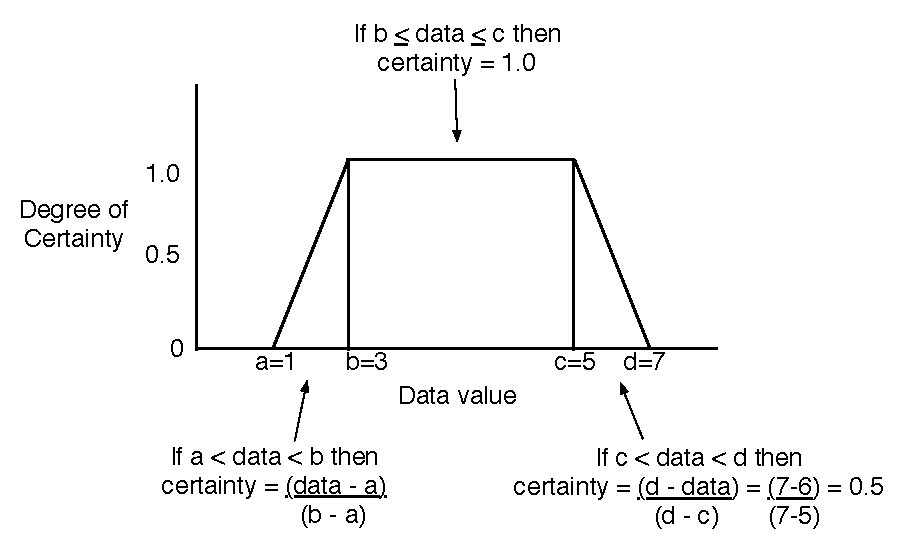
\includegraphics[width=0.95\textwidth]{../trapFigExample.pdf}
%  \end{column}

%  \begin{column}{0.4\textwidth}
%  Example:
%  \begin{itemize}
%  	\item Feature: duration (length of the activity in seconds).
%  	\item a=1, b=3, c=5, d=7
%  	\item The length of the activity is 6 seconds (between c and d).
%  	\linespace
%  	\item prob = $\frac{d-\textrm{data}}{d-c}$ = $\frac{7-6}{7-5}$ = 0.5
%  \end{itemize}

%  \end{column}
%  \end{columns}
\end{frame}


\begin{frame}
	\frametitle{Encoding of Features and Rules}
	\begin{itemize}
	\item The four parameters are encoded into blocks. Each block is a feature with values between 0 and 7.
	\end{itemize}
	
\begin{figure}
\begin{tabular}{|cccc|} \hline
010 & 011 & 100 & 101\\
a=2 & b=3 & c=4 & d=5\\
\hline\end{tabular}
\end{figure}

	\begin{itemize}
	\item A rule has one block for each of 12 features followed at the end by a marker indicating the type of attack.
	\end{itemize}

\begin{figure}
\begin{small}
\begin{tabular}{|cccc|c|cccc|c|} \hline
010 & 011 & 100 & 101   & ...... & 010 & 011 & 101 & 111   & DoS\\
a=2 & b=3 & c=4 & d=5   & ...... & a=2 & b=3 & c=5 & d=7   &\\ 
    &     & Block 1&    &        &     & Block 12& &       & Type\\
\hline\end{tabular}
\caption{Based on [Jongsuebsuk-Wattanapongsakorn-Charnsripinyo, 2013]}
\end{small}
\end{figure}

	\begin{itemize}
		\item The degree of certainty is computed for each of the 12 blocks, and if the sum of those is greater than a threshold, then it will be declared as an attack.
	\end{itemize}

\end{frame}


\subsection{Algorithm Overview}

\begin{frame}
	\frametitle{Algorithm Overview}
	\begin{itemize}
		\item One record is passed into a rule.
		\item Each feature in a record is matched to one block of the rule.
		\item The parameters of each block measure the degree of certainty of an attack using the trapezoidal fuzzy rule shape.
		\item The sum of the degrees of certainty from each block are then compared with a threshold to determine if the record represents an attack or normal behavior.
	\end{itemize}
\end{frame}

\begin{frame}
	\frametitle{Algorithm}
\begin{columns}
\begin{column}{0.6\textwidth}
\begin{small}
\begin{algorithmic}
\FOR{each rule}
  \FOR{each record}
    \FOR{each feature}
      \STATE{prob = fuzzy();}
      \STATE{totalprob = totalprob + prob;}
    \ENDFOR    
    \IF{totalprob > threshold} 
      \STATE{class is attack;}
      \ELSE \STATE{class is normal;}
    \ENDIF
  \ENDFOR
  \STATE{find $A$, $B$, $\alpha$, and $\beta$  %// $A$: \# of attack records. $B$: \# of normal records. $\alpha$: \# of attack records correctly identified as attack. $\beta$: \# of normal records incorrectly classified as attack.}
  
  } 
\ENDFOR
\STATE{calculate fitness}
\STATE{crossover(), mutation()}

\end{algorithmic}
\end{small}
\end{column}

\begin{column}{0.4\textwidth}
	The fitness function in the algorithm is:
	\begin{equation*}
	\frac{\alpha}{A} - \frac{\beta}{B}
	\end{equation*}

	$A$: \# of attack records.
	
	$B$: \# of normal records. 

	$\alpha$: \# of attack records correctly identified as attack.

	$\beta$: \# of normal records incorrectly classified as attack.
	
\end{column}
\end{columns}
\end{frame}


\subsection{Experimental Design and Results}

\begin{frame}
	\frametitle{Experiments}
	\begin{itemize}
		\item A variety of experiments were run. Two experiments used just RLD09. Three experiments used both RLD09 and KDD99 in order to compare how the fuzzy GA would perform on both.
	\end{itemize}
\end{frame}


\begin{frame}
	\frametitle{Experiments Using Only RLD09}
	Experiment 1
	\begin{itemize}
		\item Fuzzy GA was used to create DoS and probe detection rules. Both the DoS and probe rules were then used together in the testing process to identify attacks from the testing data set.
		\item 10,000 records in the training set, 26,500 records in the test set.
	\end{itemize}

\linespace
\begin{itemize}
	\item The following algorithm was used to identify attacks and normal activity in this experiment.
\end{itemize}

\begin{algorithmic}
\IF{dos\_rule = yes or probe\_rule = yes}
	\STATE{This record is an attack;}
\ELSE \STATE{This record is normal;}
\ENDIF
\end{algorithmic}
\end{frame}


\begin{frame}
	\frametitle{Experiments Using Only RLD09}
	Experiment 1 Results
\begin{table}
\begin{small}
\begin{tabular}{lllllll}
 & Attack & Normal & Total & FP(\%) & FN(\%) & DR(\%)\\
DoS Training & 1499 & 8501 & 10000 & 1.46 & 47.50 & 91.64\\
Probe Training & 2496 & 7504 & 10000 & 1.83 & 15.38 & 94.79\\
Testing & 10500 & 16000 & 26500 & 1.13 & 4.10 & 97.92\\
\end{tabular}
\end{small}
\end{table}
\end{frame}


\begin{frame}
	\frametitle{Experiments Using Only RLD09}
Experiment 2
	\begin{itemize}
		\item Attacks were pulled out of the training set and kept for unknown data testing. This was to test that the fuzzy GA could detect unknown attacks.
		\item Used fuzzy GA and a decision tree algorithm.
		\item For each test case there were 13 attack types plus normal activity that were in the training data set. Three attack types were used for the unknown testing data set.
	\end{itemize}
\end{frame}


\begin{frame}
	\frametitle{Experiments Using Only RLD09}
	Experiment 2 Results (7 tests were run in total, 5 are shown here.)
	
\begin{table}
\begin{footnotesize}
\begin{tabular}{llll}
Test & Unknown & Decision & Fuzzy\\
Case & Attacks & Tree DR (\%) & Genetic DR (\%)\\ \hline

1 & Adv Port Scan (Probe) & Avg = & Avg =\\
  & Ack Scan (Probe)                 & 98.33 & 100\\
  & Xmas Tree (Probe)                 &                 &\\ \hline

2 & UDP Flood (DoS) & Avg = & Avg =\\
  & Host Scan (Probe) & 46.65 & 99.80\\
  & UDP Scan (Probe) & &\\ \hline

3 & Jping (DoS) & Avg = & Avg =\\
  & Syn Scan (Probe) & 99.70 & 98.75\\
  & Fin Scan (Probe) & &\\ \hline

4 & UDP Flood (DoS) & Avg = & Avg =\\
  & RCP Scan (Probe) & 70.35 & 98.15\\
  & Fin Scan (Probe) & &\\ \hline

5 & Http Flood (DoS) & Avg = & Avg =\\
  & RCP Scan (Probe) & 99.94 & 97.50\\
  & Fin Scan (Probe) & &\\
\hline\end{tabular}
\end{footnotesize}
\end{table}
	
\end{frame}


\begin{frame}
	\frametitle{Experiments Using Both RLD09 and KDD99}
Experiment 1
	\begin{itemize}
		\item Used fuzzy GA to classify normal activity and attacks from KDD99 and RLD09.
	\end{itemize}
	
\begin{table}
\begin{tabular}{cccccc}
Data set & Attack & Normal & FP (\%) & FN (\%) & DR (\%)\\ \hline
KDD99 & 160,117 & 39,337 & 0.13 & 1.55 & 98.72\\
RLD09 & 10,500 & 16,000 & 1.14 & 3.39 & 97.97\\
\end{tabular}
\end{table}
\end{frame}


\begin{frame}
	\frametitle{Experiments Using Both RLD09 and KDD99}
Experiment 2
	\begin{itemize}
		\item Used the fuzzy GA to classify types of attacks in KDD99.
		\item 158,597 records of DoS attacks. 1,500 records of probe attacks.
		\item 10 tests were run in total, 5 are shown here.
	\end{itemize}
\begin{table}
\begin{tabular}{cccccc}
Test & Attack & Type & FP (\%) & FN (\%) & DR (\%)\\ \hline
1 & Back & DoS & 85.33 & 0.00 & 16.56\\
2 & Smurf & DoS & 0.76 & 0.10 & 99.73\\
3 & Neptune & DoS & 0.15 & 0.34 & 99.75\\
4 & Portsweep & Probe & 6.40 & 0.00 & 93.66\\
5 & Satan & Probe & 0.74 & 3.75 & 99.22\\
\end{tabular}
\end{table}

\end{frame}


\begin{frame}
	\frametitle{Experiments Using Both RLD09 and KDD99}
Experiment 3
	\begin{itemize}
		\item Used the fuzzy GA to classify types of attacks in RLD09.
		\item 6,400 records of DoS attacks. 10,400 records of probe attacks.
		\item 17 tests were run in total, 6 are shown here.
	\end{itemize}
\begin{table}
\begin{tabular}{cccccc}
Test & Attack & Type & FP (\%) & FN (\%) & DR (\%)\\ \hline
1 & HTTP Flood & DoS & 0.36 & 3.5 & 99.46\\
2 & Smurf & DoS & 0.02 & 0 & 99.98\\
3 & UDP Flood & DoS & 11.06 & 0 & 89.59\\
4 & Fin Scan & Probe & 2.58 & 0 & 97.50\\
5 & IP Scan & Probe & 13.01 & 16.4 & 86.89\\
6 & Syn Scan & Probe & 0.65 & 4.2 & 99.24\\
\end{tabular}
\end{table}

\end{frame}
%%%%%%%%%%%%%%%%%%%%%%%%%%%%%%%%%%%%%%%%%%%%%%%%%%%%%%%%%%%%%%%%%%%%%%%%%%%%%%%%%
%%%%%%%%%%%%%%%%%%%%%%%%%%%%%%%%%%%%%%%%%%%%%%%%%%%%%%%%%%%%%%%%%%%%%%%%%%%%%%%%%
%%%%%%%%%%%%%%%%%%%%%%%%%%%%%%%%%%%%%%%%%%%%%%%%%%%%%%%%%%%%%%%%%%%%%%%%%%%%%%%%%
%%%%%%%%%%%%%%%%%%%%%%%%%%%%%%%%%%%%%%%%%%%%%%%%%%%%%%%%%%%%%%%%%%%%%%%%%%%%%%%%%
\section[Conclusions]{Conclusions}

\begin{frame}
\frametitle{Conclusions}
	\begin{itemize}
		\item The fuzzy genetic algorithm had a higher detection rate than a decision tree algorithm in most cases.
		\item Fuzzy genetic algorithms are good at detecting unknown attacks.
		\item The use of fuzzy genetic algorithms in intrusion detection is an effective way of detecting attacks.
	\end{itemize}
\end{frame}


\begin{frame}
	\frametitle{Thanks!}
	
	Thank you for your time and attention!
		
	\linespace
	\linespace
	
	\begin{center}
	{\huge Questions?}
	\end{center}
\end{frame}

\section*{References}

\begin{frame} 
	\frametitle{References} 
	
	\begin{thebibliography}{lskdjf}
	
	\begin{small}
	\bibitem{6496342}
Jongsuebsuk, P. and Wattanapongsakorn, N. and Charnsripinyo, C.
\newblock Network intrusion detection with Fuzzy Genetic Algorithm for unknown attacks.
\newblock In \emph{2013 International Conference on Information Networking (ICOIN)}, pages 1-5, 2013.
	
	
	\bibitem{6559603}
Jongsuebsuk, P. and Wattanapongsakorn, N. and Charnsripinyo, C.
\newblock Real-time intrusion detection with fuzzy genetic algorithm.
\newblock In \emph{2013 10th International Conference on Electrical Engineering/Electronics, Computer, Telecommunications and Information Technology (ECTI-CON)}, pages 1-6, 2013.
	
	
%	\bibitem{DBLP:journals/corr/abs-1204-1336}
%Mohammad Sazzadul Hoque, Md. Abdul Mukit, Md. Abu Naser Bikas.
%\newblock An Implementation of Intrusion Detection System Using Genetic Algorithm.
%\newblock \emph{CoRR}, abs/1204.1336, 2012.
	\end{small}
	
  	\end{thebibliography}
  	
  	\linespace
  	
  	\begin{center}
  	\begin{small}
  	See my Senior Seminar paper for additional references.
  	\end{small}
  	\end{center}
	
\end{frame} 

\end{document}


